% Source: Code/DualStemFCNN_IR_RGB/pipeline3.tex

\documentclass[border=4pt]{standalone}
\usepackage{tikz}
\usepackage{xcolor}
\usetikzlibrary{positioning,shapes,arrows.meta,calc}

\definecolor{garnet}{HTML}{73000A}
\definecolor{black90}{HTML}{363636}
\definecolor{black70}{HTML}{5C5C5C}
\definecolor{black50}{HTML}{A2A2A2}
\definecolor{black30}{HTML}{C7C7C7}
\definecolor{black10}{HTML}{ECECEC}
\definecolor{warmgrey}{HTML}{676156}
\definecolor{sandstorm}{HTML}{FFF2E3}
\definecolor{rose}{HTML}{CC2E40}
\definecolor{atlantic}{HTML}{466A9F}
\definecolor{congaree}{HTML}{1F414D}
\definecolor{horseshoe}{HTML}{65780B}
\definecolor{grass}{HTML}{CED318}
\definecolor{honeycomb}{HTML}{A49137}

\begin{document}
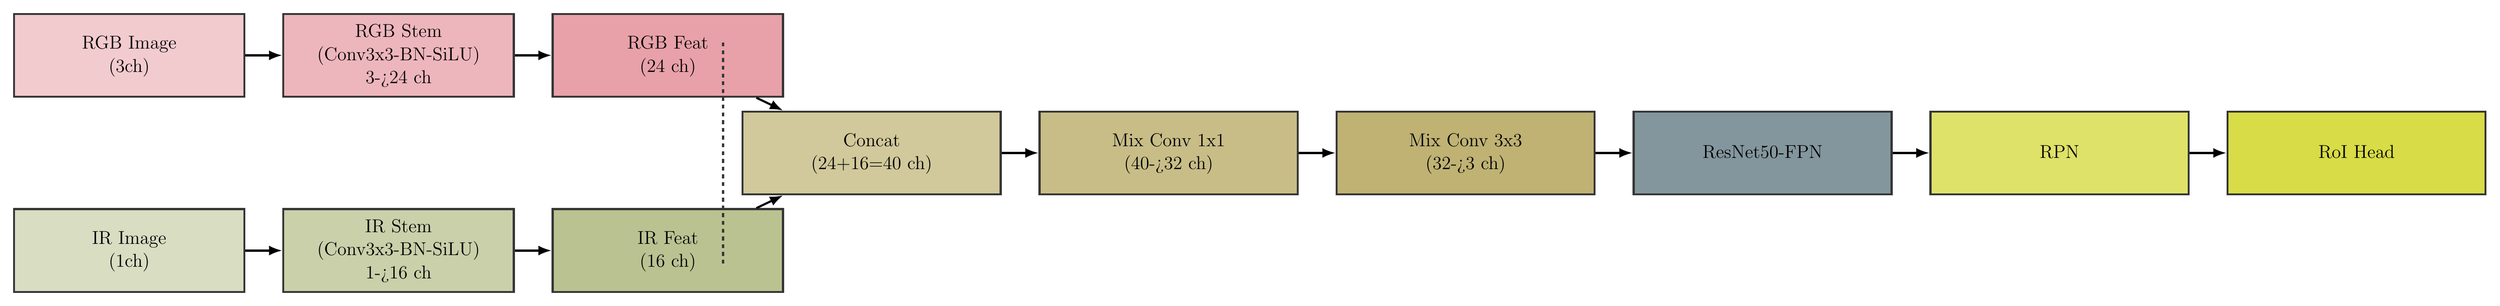
\begin{tikzpicture}[
    box/.style={rectangle, draw=black90, ultra thick, minimum width=6.25cm, minimum height=2.25cm, align=center, font=\Large, text depth=0.5ex}, % Added text depth
    arrow/.style={-Latex, ultra thick, draw=black}
]
    % RGB branch
    \node[box, fill=rose!25] (rgb_img) {RGB Image\\(3ch)};
    \node[box, fill=rose!35, right=of rgb_img] (rgb_stem) {RGB Stem\\(Conv3x3-BN-SiLU)\\3->24 ch};
    \node[box, fill=rose!45, right=of rgb_stem] (rgb_feat) {RGB Feat\\(24 ch)};
    
    % IR branch (aligned below)
    \node[box, fill=horseshoe!25, below=30mm of rgb_img] (ir_img) {IR Image\\(1ch)};
    \node[box, fill=horseshoe!35, right=of ir_img] (ir_stem) {IR Stem\\(Conv3x3-BN-SiLU)\\1->16 ch};
    \node[box, fill=horseshoe!45, right=of ir_stem] (ir_feat) {IR Feat\\(16 ch)};
    
    % Fusion (centered between branches)
    \node[box, fill=honeycomb!50, right=2cm of $(rgb_feat)!0.5!(ir_feat)$, minimum width=7cm] (concat) {Concat\\(24+16=40 ch)};
    \node[box, fill=honeycomb!60, right=of concat, minimum width=7cm] (mix1) {Mix Conv 1x1\\(40->32 ch)};
    \node[box, fill=honeycomb!70, right=of mix1, minimum width=7cm] (mix2) {Mix Conv 3x3\\(32->3 ch)};
    
    % Single pipeline
    \node[box, fill=congaree!55, right=of mix2, minimum width=7cm] (backbone) {ResNet50-FPN};
    \node[box, fill=grass!65, right=of backbone, minimum width=7cm] (rpn) {RPN};
    \node[box, fill=grass!80, right=of rpn, minimum width=7cm] (detector) {RoI Head};
    
    % Arrows: RGB branch
    \draw[arrow] (rgb_img) -- (rgb_stem);
    \draw[arrow] (rgb_stem) -- (rgb_feat);
    \draw[arrow] (rgb_feat) -- (concat);
    
    % Arrows: IR branch
    \draw[arrow] (ir_img) -- (ir_stem);
    \draw[arrow] (ir_stem) -- (ir_feat);
    \draw[arrow] (ir_feat) -- (concat);
    
    % Arrows: fused pipeline
    \draw[arrow] (concat) -- (mix1);
    \draw[arrow] (mix1) -- (mix2);
    \draw[arrow] (mix2) -- (backbone);
    \draw[arrow] (backbone) -- (rpn);
    \draw[arrow] (rpn) -- (detector);
    
    % Vertical separator showing the dual-to-single merge
    \draw[dashed, black90, ultra thick] ($(concat.west)+(-5mm, 3cm)$) -- ($(concat.west)+(-5mm, -3cm)$);
\end{tikzpicture}
\end{document}
